% 

\begin{frame}{Structure of the talk}
\begin{itemize}
  \item Post-quantum WireGuard\footnote{
	  Andreas Hülsing, Kai-Chun Ning, Peter Schwabe, Florian Weber, and Philip R. Zimmermann. “Post-quantum WireGuard”. In: 42nd IEEE Symposium on Security and Privacy, SP 2021, San Francisco, CA, USA, 24-27 May 2021. Full version: https://eprint.iacr.org/2020/379
	}: How to build an interactive key exchange from KEMs
  \item Contribution: State Disruption Attacks \& cookies as a defense
  \item Contribution: New hashing \& domain separation scheme
  \item Contribution: Symbolic analysis of the Rosenpass protocol
  \item Contribution: Reference implementation – Securing WireGuard in practice
  \item Contribution: Noise-like specification
\end{itemize}
\end{frame}

\begin{frame}{Post-quantum WireGuard: Three encapsulations}
\tikzset{shorten > = 1pt,shorten < = 1pt}
\begin{columns}

\begin{column}{.30\textwidth}
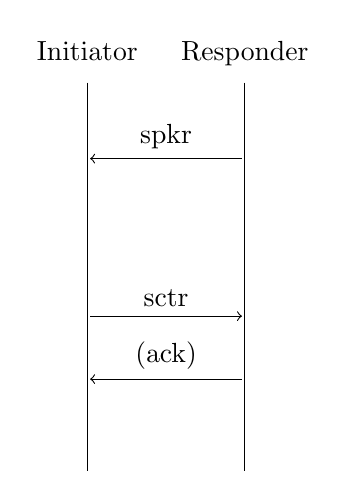
\begin{tikzpicture}
	 \draw (-1,0) node[above](initiator){Initiator\strut} --
		coordinate[pos=.2](spkr-y)
		coordinate[pos=.6](sctr-y)
		coordinate[pos=.76](ack-y)+(0,-5);
	  \draw (1,0) node[above](responder){Responder\strut}-- +(0,-5);


		\draw[<-](spkr-y-|initiator) -- node[above]{spkr} (spkr-y-|responder);
		\draw[->](sctr-y-|initiator) -- node[above] {sctr} (sctr-y-|responder);
		\draw[<-](ack-y-|initiator) -- node[above] {(ack)} (ack-y-|responder);

\end{tikzpicture}
Responder Auth
\end{column}

\begin{column}{.30\textwidth}
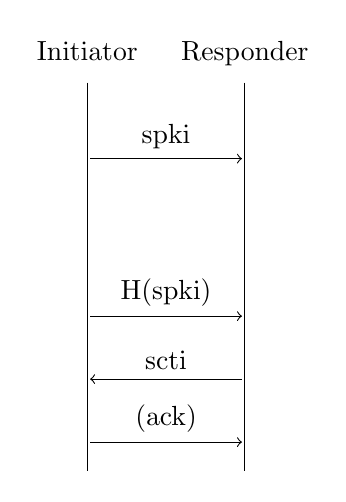
\begin{tikzpicture}
	 \draw (-1,0) node[above](initiator){Initiator\strut} --
		coordinate[pos=.2](spki-y)
		coordinate[pos=.6](Hspki-y)
		coordinate[pos=.76] (scti-y)
		coordinate[pos=.92](ack-y)+(0,-5);
	 \draw (1,0) node[above](responder){Responder\strut}-- +(0,-5);

	 \draw[->](spki-y-|initiator) -- node[above]{spki} (spki-y-|responder);
	 \draw[->](Hspki-y-|initiator) -- node[above] {H(spki)} (Hspki-y-|responder);

	  \draw[<-](scti-y-|initiator) -- node[above]{scti} (scti-y-|responder);

	 \draw[->](ack-y-|initiator) -- node[above] {(ack)} (ack-y-|responder);

\end{tikzpicture}
Initiator Auth
\end{column}

\begin{column}{.30\textwidth}
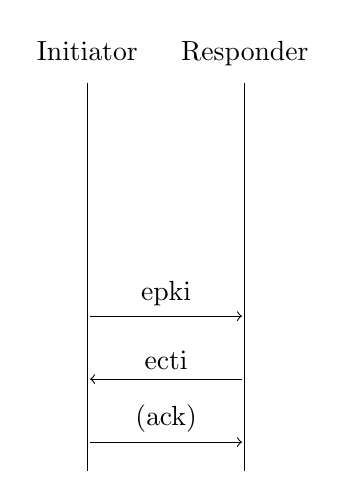
\begin{tikzpicture}
	 \draw (-1,0) node[above](initiator){Initiator\strut} --
		coordinate[pos=.6](epki-y)
		coordinate[pos=.76] (ecti-y)
		coordinate[pos=.92](ack-y)+(0,-5);
	 \draw (1,0) node[above](responder){Responder\strut}-- +(0,-5);

	 \draw[->](epki-y-|initiator) -- node[above]{epki} (epki-y-|responder);
	 \draw[<-](ecti-y-|initiator) -- node[above]{ecti} (ecti-y-|responder);
	 \draw[->](ack-y-|initiator) -- node[above] {(ack)} (ack-y-|responder);

\end{tikzpicture}
Forward secrecy
\end{column}

\end{columns}
\end{frame}

\begin{frame}{Combining the three encapsulations in one protocol}

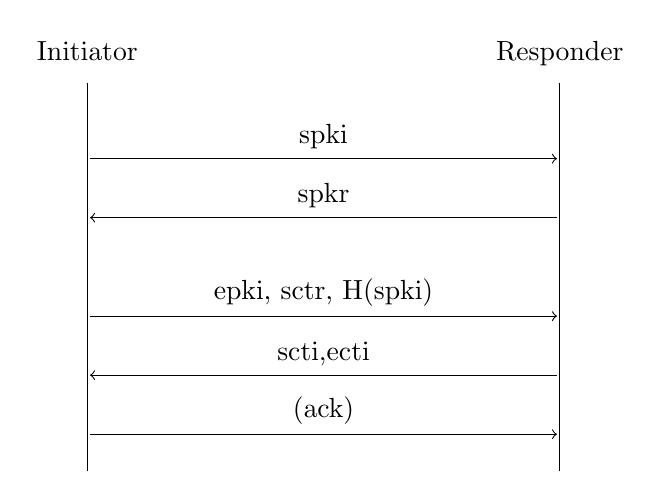
\begin{tikzpicture}[shorten > = 1pt,shorten < = 1pt]
	\draw (-3,0) node[above](initiator){Initiator\strut} -- coordinate[pos=.2](spki-y)
	coordinate[pos=.35](spkr-y)
	coordinate[pos=.6](epki-y)
	coordinate[pos=.75](scti-y)
	coordinate[pos=.9](ack-y)+(0,-5);
	\draw (3,0) node[above](responder){Responder\strut}-- +(0,-5);

	 \draw[->](spki-y-|initiator) -- node[above] {spki} (spki-y-|responder);
	 \draw[<-](spkr-y-|initiator) -- node[above] {spkr} (spkr-y-|responder);
	 \draw[->](epki-y-|initiator) -- node[above] {epki, sctr, H(spki)} (epki-y-|responder);
	 \draw[<-](scti-y-|initiator) -- node[above] {scti,ecti} (scti-y-|responder);
	  \draw[->](ack-y-|initiator) -- node[above] {(ack)} (ack-y-|responder);

\end{tikzpicture}

  Note that the initiator is not authenticated until they send \enquote{(ack)}.

\end{frame}

\begin{frame}{The Rosenpass protocol}
  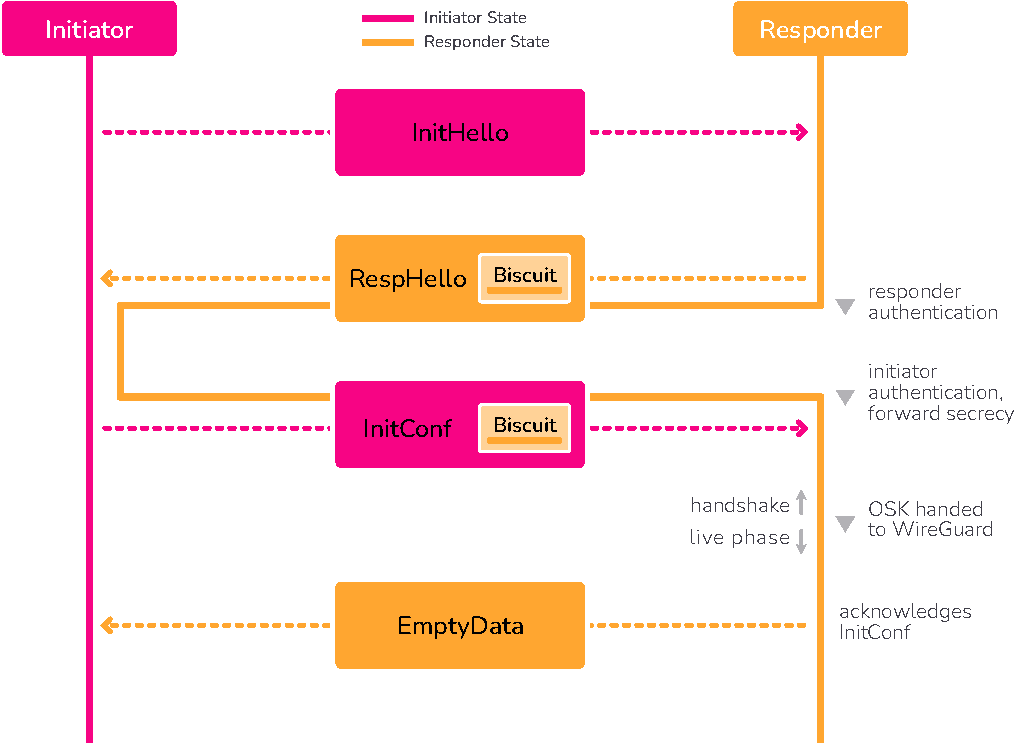
\includegraphics[height=.9\textheight]{graphics/rosenpass-wp-key-exchange-protocol-rgb.pdf}
\end{frame}

\begin{frame}{CVE-2021-46873 – DOS against WireGuard through NTP}
\begin{itemize}
  \item The replay protection in classic WireGuard assumes a monotonic counter
  \item But the system time is attacker controlled because NTP is insecure
  \item This generates a kill packet that abuses replay protection and renders the initiator's key-pair useless
  \item Attack is possible in the real world!
  \item Similar attack in post-quantum WireGuard is worse since InitHello is unauthenticated
  \item Solution: Biscuits
\end{itemize}
\end{frame}

\begin{frame}{New Hashing/Domain separation scheme}
  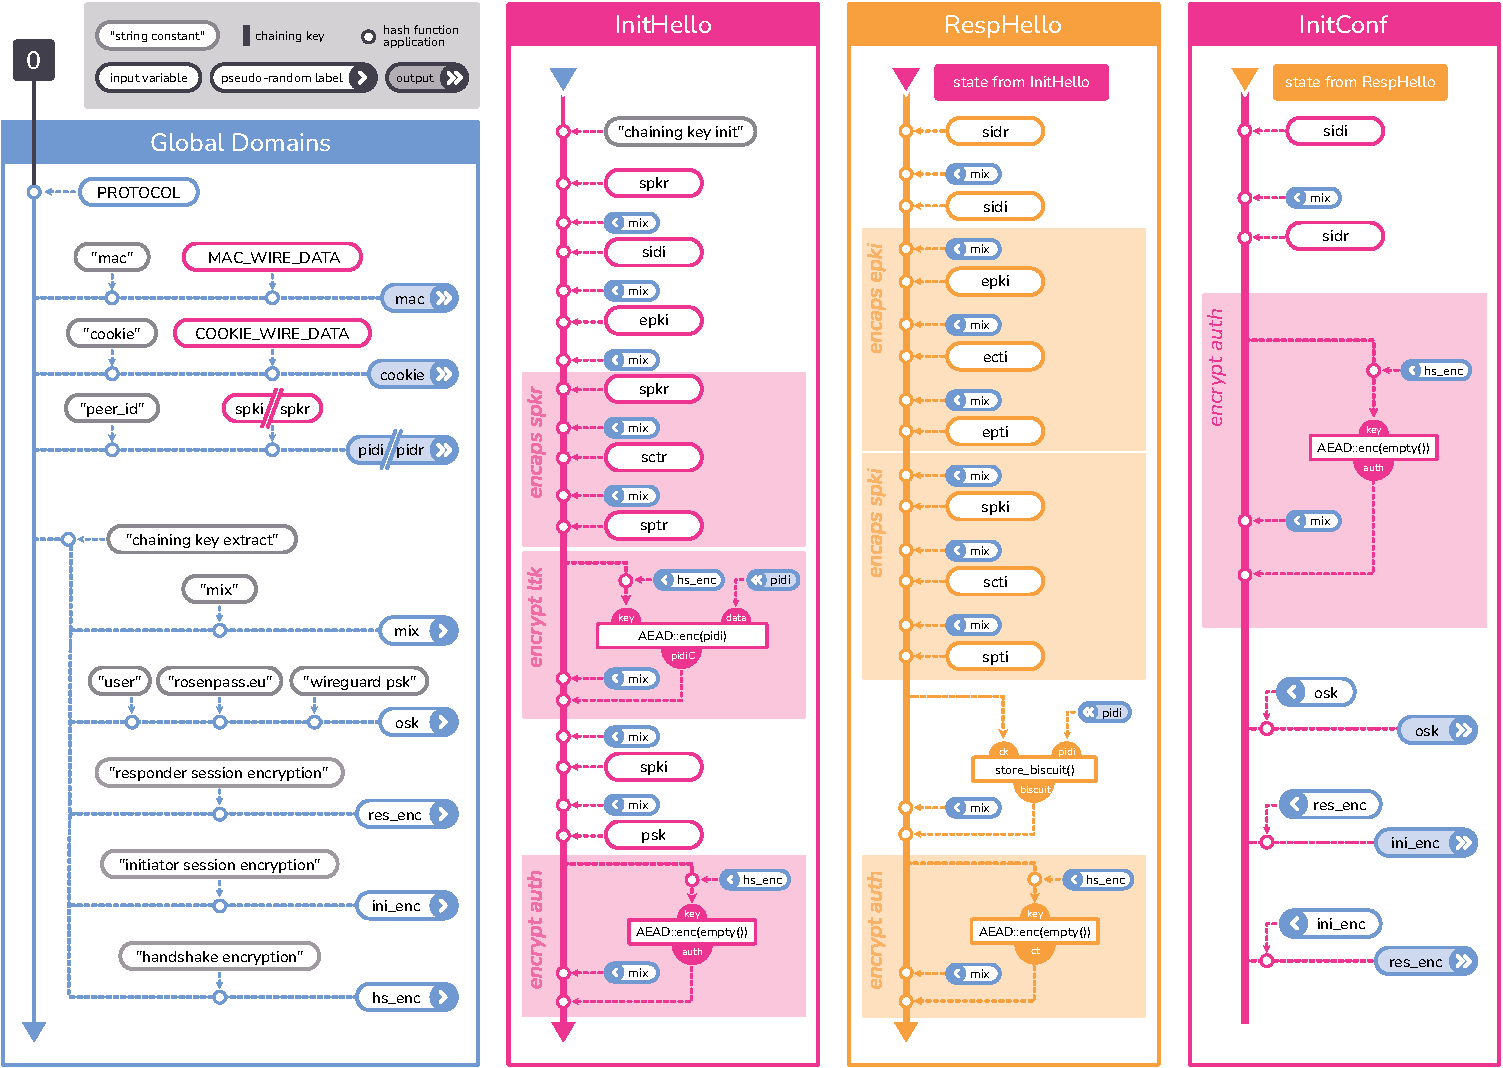
\includegraphics[height=.9\textheight]{graphics/rosenpass-wp-hashing-tree.pdf}
\end{frame}

\begin{frame}{Security analysis of rosenpass}
  \begin{itemize}
	\item CryptoVerif in progress
	\item Symbolic analysis using ProVerif
  \item Code is part of the software repository \& build system
  \item Symbolic analysis is fast (about five minutes), runs in parallel and is
  \end{itemize}
\end{frame}

\begin{frame}{Proverif in technicolor}
  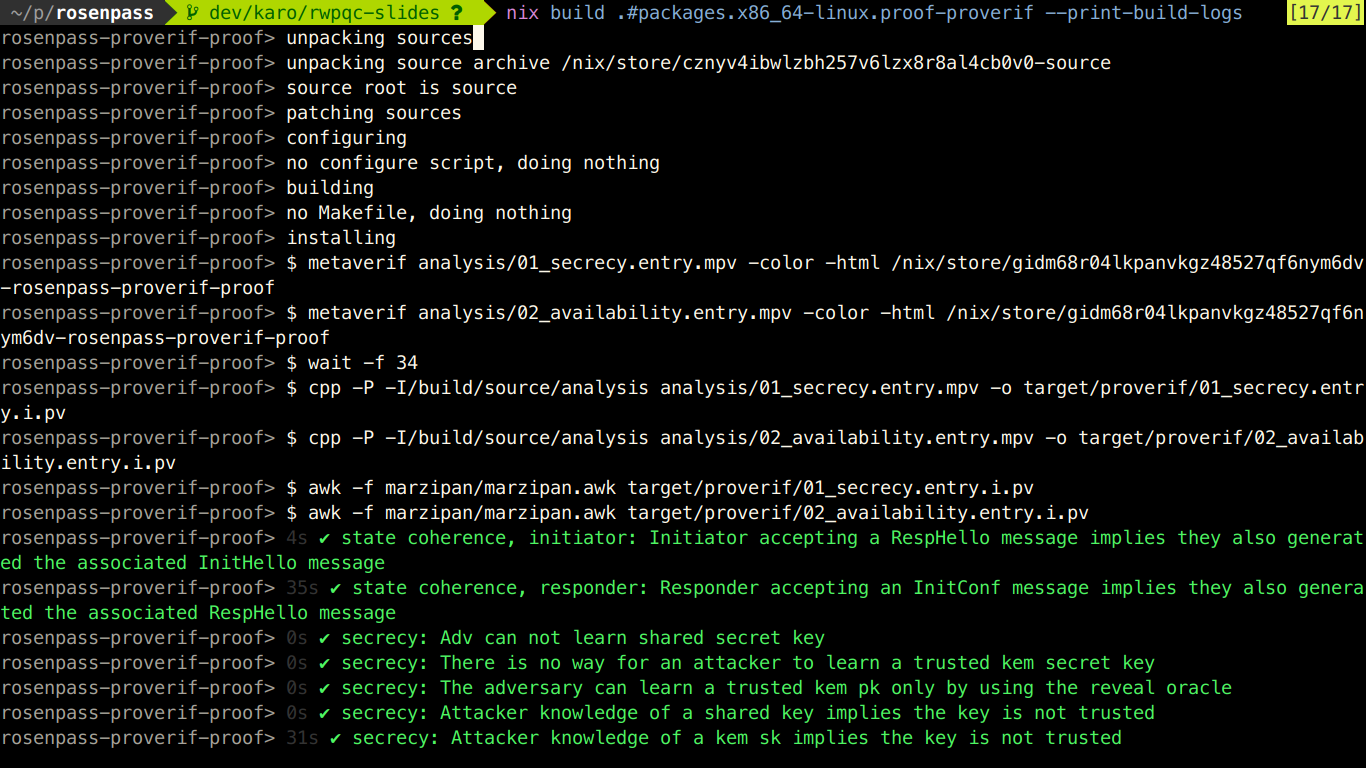
\includegraphics[height=.9\textheight]{assets/2023-03-20-symbolic-analysis-screenshot.png}
\end{frame}

\begin{frame}{Reference implementation in rust, deploying post-quantum-secure WireGuard}
  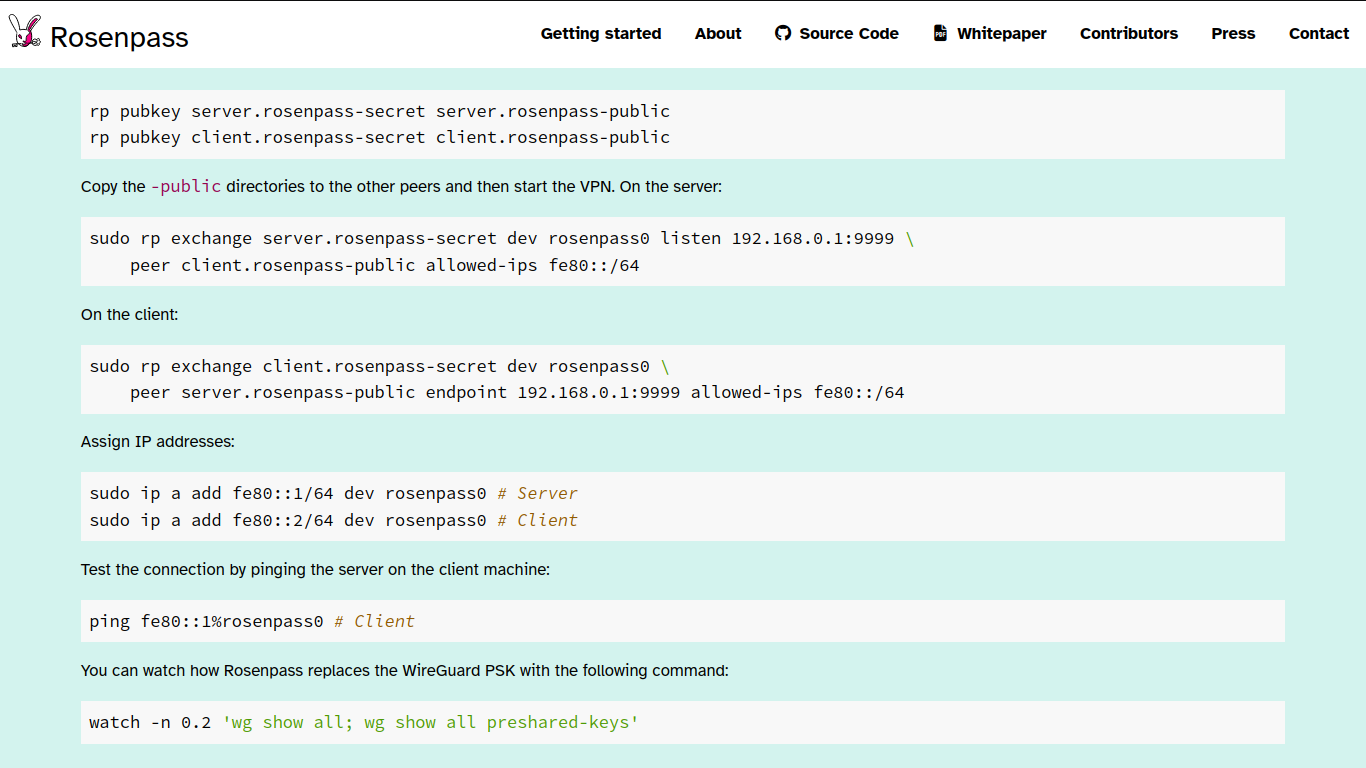
\includegraphics[height=.9\textheight]{assets/2023-03-20-rg-tutorial-screenshot.png}
\end{frame}

\begin{frame}{Noise-like specification (easier for engineers)}
  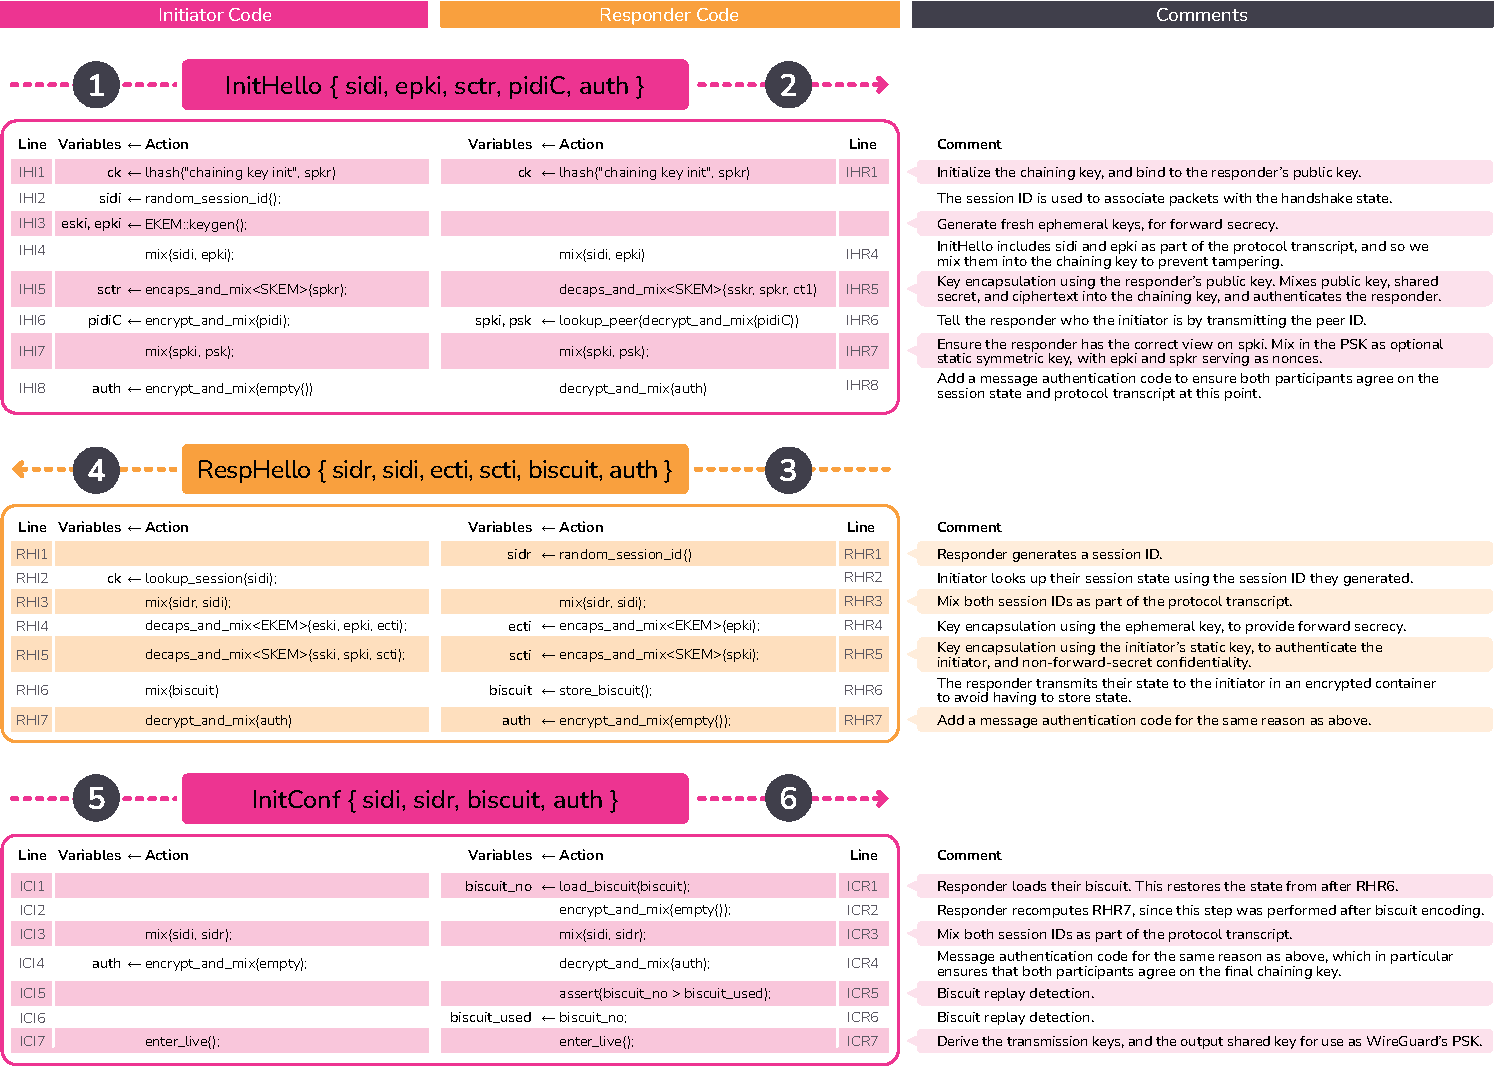
\includegraphics[height=.9\textheight]{graphics/rosenpass-wp-message-handling-code.pdf}
\end{frame}
